\documentclass[a4paper]{article}

%% Language and font encodings
\usepackage[brazil,english]{babel}
\usepackage[utf8]{inputenc}
\usepackage[T1]{fontenc}

%% Sets page size and margins
\usepackage[a4paper,top=3cm,bottom=2cm,left=3cm,right=3cm,marginparwidth=1.75cm]{geometry}

%% Useful packages
\usepackage{amsmath}
\usepackage{graphicx}
\usepackage[colorinlistoftodos]{todonotes}
\usepackage[colorlinks=true, allcolors=blue]{hyperref}

\title{Simulação e jogo com mapas de influência}
\author{Diego Cardozo Sandrim}

\begin{document}
\maketitle

\begin{abstract}
Mapas de influência são utilizados em jogos e simulações para representar inteligência artificial de agentes. São apresentados um jogo e uma simulação que usam essa técnica em conjunto com otimizações como o limite de influência. A simulação pode ser utilizada para projetar um vagão de trem e testar como as pessoas se comportam dentro dele antes que o vagão seja construído. O jogo mostra uma combinação de múltiplos mapas de influência com arvores de decisão para se aproximar ao comportamento inteligente.
\end{abstract}

\section{Introdução}

Jogos de computador e simulações podem utilizar mapas de influência para simular comportamento inteligente de agentes. Mapa de influência é uma matriz de dados que representa a influência de cada agente em um campo. \cite{Millington:2009:AIG:1795711}

A matriz de influência é populada com os dados de cada agente que está em um campo. Cada agente pode ter um valor intrínseco de influência, e quanto mais perto do agente o item da matriz está, mais forte é a influência que ele causa naquele item. Somando-se todos os valores de influência dos agentes para uma célula temos a influência completa da matriz.

O valor da influência que um agente causa em função da sua distancia até célula que está sendo calculada pode ser variar para que a influência do agente chegue longe com valores altos, ou caia rapidamente nas células vizinhas, dessa forma podemos das diferentes funções de decaimento de influência para cada agente em campo.

Matrizes de influência são caras computacionalmente pois tem complexidade de $O(N.M.A)$, onde $N$ é o número de colunas da matriz, $M$ o número de linhas e a o número de agentes. Por esse motivo é comum construir simplificações para calcular a matriz, mesmo que isso tenha impacto na precisão dos dados.

Uma das formas de simplificar o calculo da matriz de influência é limitar o quão distante a influência de um agente pode chegar. Com esse método a complexidade fica em $O(I.A)$, onde $I$ é a quantidade de células onde o agente oferece influência, que deve ser menor que $N.M$. Uma desvantagem desse método é que uma numerosa quantidade de agentes poderia causar uma forte influência a uma certa distancia, mas se essa distancia for menor que o raio usado na simplificação, a influência será desconsiderada.

\section{Aplicações}

No presente trabalho a técnica de mapas de influência foi aplicada a dois sistemas. O primeira se refere a uma simulação de embarque de passageiros em um vagão de trem. O segundo trata-se de um jogo popularmente conhecido como rouba-bandeira. Os dois cenários foram desenvolvidos na linguagem Lua, com o \textit{framework} LÖVE.

\subsection{Simulação de embarque}

\subsubsection{Público alvo}

A simulação de embarque de trem tem como público alvo projetistas de trens. Eles poderiam se beneficiar dessa simulação para testar como as pessoas se comportariam em um modelo de vagão sendo projetado. Os testes podem revelar medidas sobre qual o tempo de embarque, qual percurso as pessoas fazem entre a porta e o local onde se acomodam, onde as pessoas se concentrariam e qual a probabilidade de choque entre passageiros.

\subsubsection{Apresentação}

O cenário se trata de uma plataforma de embarque, com um vagão de trem com as portas abertas. O vagão é formado por suas paredes, espaços abertos representando as portas assentos vazios dentro do vagão. Diversos usuários estão na plataforma. Assim que o jogo começa os usuários iniciam a movimentação. Existem objetos invisíveis que representam a plataforma e os espaços do trem onde os usuários podem ficar em pé.

\begin{figure}
\centering
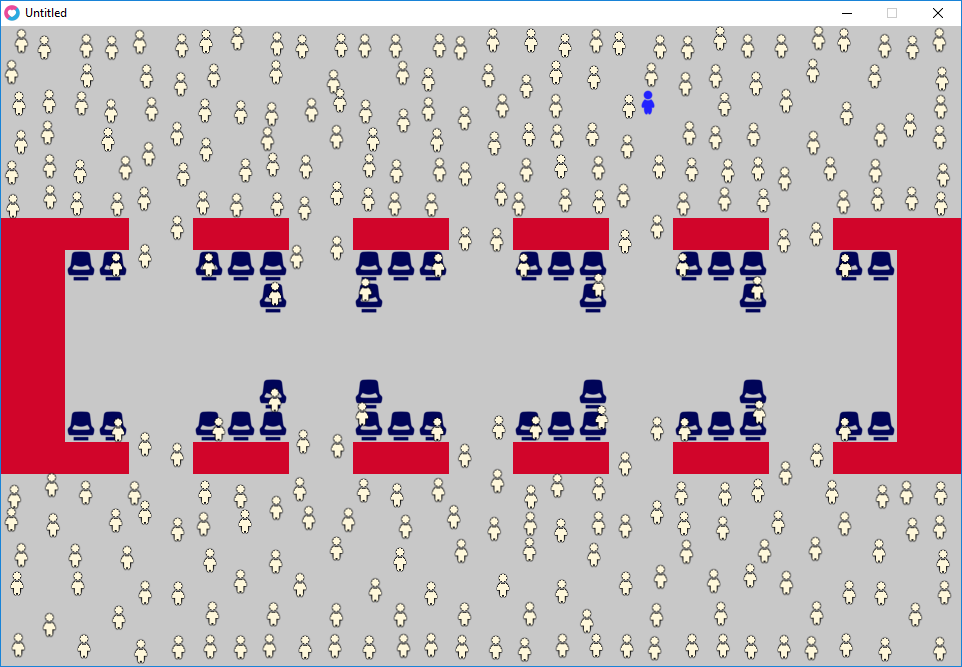
\includegraphics[width=1\textwidth]{train.png}
\caption{\label{fig:train} Início da simulação de embarque.}
\end{figure}

\subsubsection{Descrição técnica}

O jogo contém alguns controles de teclado para o projetista avaliar melhor o cenário. O botão $p$ pausa e continua o jogo. O botão $d$ habilita ou desabilita o modo de depuração, onde é mostrado o mapa de influência. Quando está pausado o botão $s$ faz a simulação rodar pequenos passos enquanto está pressionado. O botão $r$ reinicia a simulação. Os botões $+$ e $-$ controlam a velocidade da simulação. Além disso há um usuário especial em uma cor diferenciada que o projetista pode controlar por todo o cenário com as setas do teclado.

Cada um dos itens do cenário exerce influência. Assentos e vagas em pé no vagão tem influência numericamente positiva, ou seja, atraem os usuários. Usuários, a plataforma de embarque e as paredes do trem tem influência numericamente negativa, dessa forma afastam os usuários.

A posição onde o vagão e seus componentes se encontra é fixa, os usuários são colocados aleatoriamente fora do vagão. Em cada laço do jogo um novo mapa de influência é calculado, cada um dos usuários consulta o mapa de influência e verifica para onde deve ir. Nenhuma rota é traçada, o usuário sempre escolhe em qual direção seguir consultando as 9 células mais próximas dele, a sua própria célula e mais as suas 8 vizinhas.

Foi utilizado o método de limite do raio de ação da influência. Cada um dos tipos itens da simulação tem valores de influência, raio, velocidade de perca de influência com o espaço. Nenhum algoritmo de detecção de influência foi usado, o mapa de influência foi suficiente para evitar colisões. Isso foi feito colocando valores altos de influência para os usuários e para as paredes do trem, juntamento com valores altos de perca de influência com a distancia.

A função de influência pela distancia utilizada foi:
\[I_{obj} = \frac{obj.influence}{(distance + 1) ^{obj.influenceDecay}}\]

Cada um dos objetos da simulação podem ter valores diferentes para influência e decaimento de influência, permitindo dessa forma a adaptação do modelo para refletir a realidade observada na plataforma.

Alguns problemas surgiram durante a implementação e foram resolvidos com soluções simples. Algumas vezes os usuários entram em um laço de movimento, esse problema aparece quando vários usuários próximos estão mudando de célula ao mesmo tempo. Esse problema costuma aparecer na vida real também quando duas pessoas tentam desviar o caminho uma da outra e acabam escolhendo o mesmo lado, e ao perceber isso as duas escolhem o outro lado novamente. No jogo esse problema foi resolvido com uma variável aleatória onde há 5\% de chance do usuário ficar parado em cada loop do jogo.

Na primeira versão do jogo houve um problema de performance ao se escolher o algoritmo incorreto para o calculo da matriz de influência. O problema consistia no fato de que a matriz de influência era calculada percorrendo-se todos os itens da matriz e para cada um dele consultar a influência que cada item da tela causa naquele ponto. Essa abordagem é ineficiente pois não permite aproveitar a limitação de distancia da influência de cada agente. Na segunda versão do algoritmo a regra foi implementada iterando-se a lista de objetos da tela e dentro desse laço escolhendo apenas as posições da matriz que estão no raio de influência do agente.

\begin{figure}
\centering
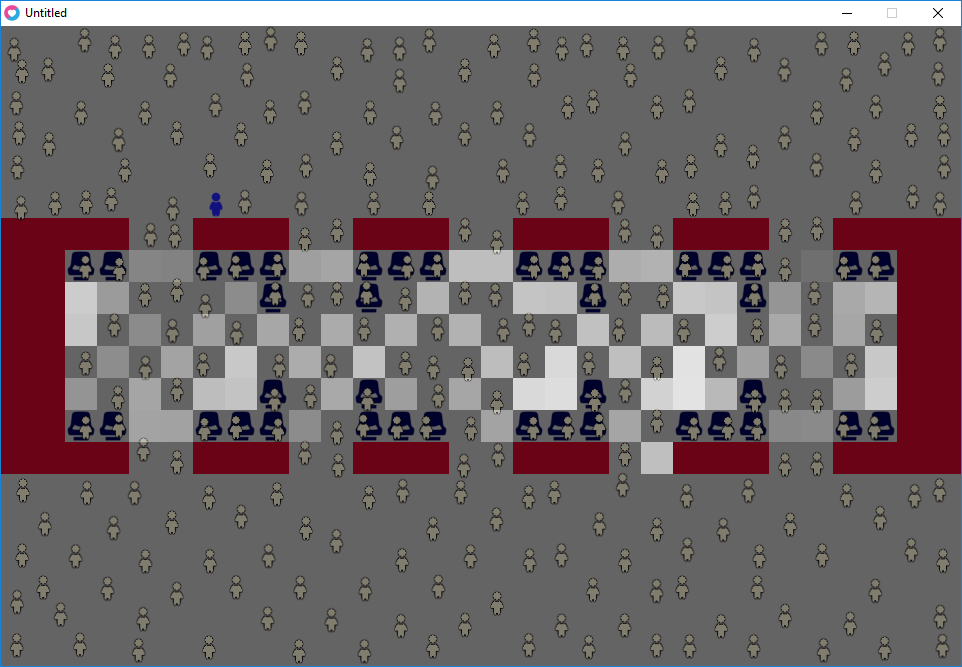
\includegraphics[width=1\textwidth]{influence-map.png}
\caption{\label{fig:influence-map} Visualização do mapa de influência}
\end{figure}

\subsubsection{Suposições}

O arquivo \textbf{parameter.lua} contém todas as parametrizações possíveis para o sistema. Nesse arquivo podemos ver as suposições realizadas:

\begin{itemize}
\item Usuário tende a ficar longe de outros usuários;
\item Usuário prefere ficar sentado do que em pé;
\item Assentos oferecem grande atratividade, porém apenas para quem está nele;
\item Lugares de pé se propagam por muitos espaço, visto que todas as pessoas querem entrar no trem;
\end{itemize}

É importante parametrizar esses valores com dados reais de como as pessoas se comportam. Utilizando vídeos gravados de dentro da plataforma, e comparando o comportamento da simulação com o comportamento real podemos obter dados fiéis do comportamento da pessoa, e dessa forma ser uma ferramenta mais precisa para o projetista.

\subsubsection{Atividades futuras}

Alguns itens podem ser melhorados no jogo

\begin{itemize}
\item Parâmetros reais, extraídos de vídeos com comportamento humano sobre o embarque.
\item Alterar a influência de um objeto uma vez que ele muda de estado.Uma vez que o assento está ocupado a influência que ele causa no mapa deve ser alterada.
\item Tipos de assentos. Adicionar assentos preferenciais às opções de assentos.
\end{itemize}

\subsection{Jogo rouba-bandeira}

\subsubsection{Público alvo}

O jogo de rouba-bandeira tem como público alvo pessoas que querem se divertir jogando um jogo virtual. É uma demonstração da utilização de múltiplos mapas de influência em conjunto com arvores de decisões simples.

\subsubsection{Apresentação}
Esse jogo consiste de dois grupos que cada um tem uma bandeira e o objetivo de cada grupo é pegar a bandeira do outro grupo e levar até sua base. O campo é dividido em dois e cada grupo tem uma parte do campo. Se um jogador está dentro do campo adversário, então ele pode ser imobilizado pelo adversário, bastando que esse toque nele.
O jogo digital tem um jogador como o próprio usuário, podendo controlá-lo para participar da partida.

\begin{figure}
\centering
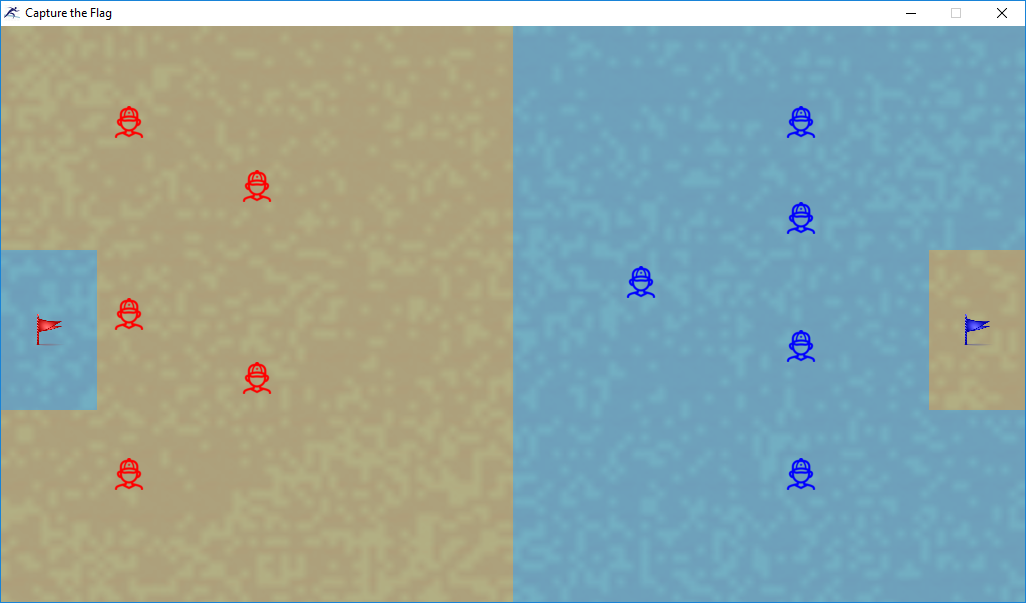
\includegraphics[width=1\textwidth]{capture-the-flag.png}
\caption{\label{fig:capture-the-flag} Tela inicial do jogo rouba-bandeira.}
\end{figure}

\subsubsection{Descrição técnica}
O jogo consiste da mesma base técnica da simulação, há objetos estáticos, como o campo, e objetos móveis como os jogadores e a bandeira. Cada tipo de objeto tem uma influência, alcance e função de decaimento própria.

Os jogadores podem estar em dois estados: ataque e defesa. No modo de ataque o jogador vai até o campo inimigo para tentar capturar a bandeira. No modo defesa o jogador tenta proteger a própria bandeira. Cada modo usa um mapa de influência diferente.

Quando um jogador consegue chegar à base inimiga e pegar a bandeira, ele se torna um objeto diferente para o mapa de influência, tento uma influência muito maior que os jogadores que não estão com a bandeira.

\subsubsection{Suposições}
Nesse jogo foi suposto:

\begin{itemize}
\item Valores e distâncias arbitrárias para a influência de cada jogador;
\item Que o jogador tem apenas o modo de ataque e de defesa;
\item Que o jogador escolhe aleatoriamente a hora de atacar;
\end{itemize}

\subsubsection{Atividades futuras}

Analisar como um jogador real se comporta segundo o mapa de influência para que possa se ajustar as parametrizações de influência de cada item da tela pode levar a um sistema de aprendizado por mapa de influência, capaz de aprender com bons jogadores e aumentar dinamicamente a dificuldade do jogo, deixando ele mais interessante.


\bibliographystyle{plain}
\bibliography{sample}

\end{document}